\documentclass[12pt,a4paper]{report}
\usepackage[latin1]{inputenc}
\usepackage[spanish]{babel}
\usepackage{graphicx}
\usepackage{kpfonts}
\usepackage{amsmath}
\usepackage{amsfonts}
\usepackage{amssymb}
\usepackage[left=2cm,right=2cm,top=2cm,bottom=2cm]{geometry}
\author{Jorge Heriberto Bueno Gomez 
4 B Ing. Mecatronica}
\title{$$Universidad Politecnica   $$
$$de la$$
$$Zona Metropolitana de Guadalajara$$
(Practica 1)
}

\begin{document}
\section{Rectificador de media onda con carga RL}
\subsection{Circuito}
$$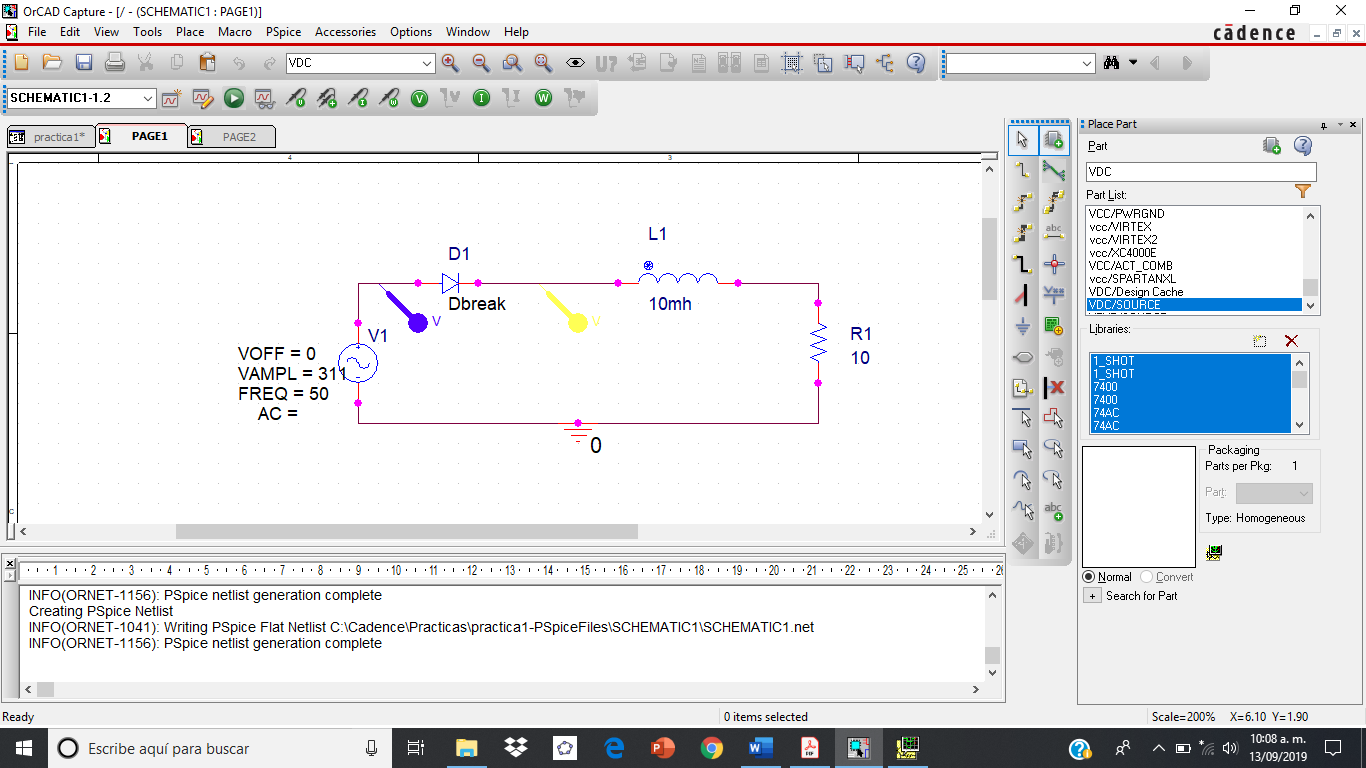
\includegraphics[scale=.25]{1.png} $$
\subsection{Onda}
$$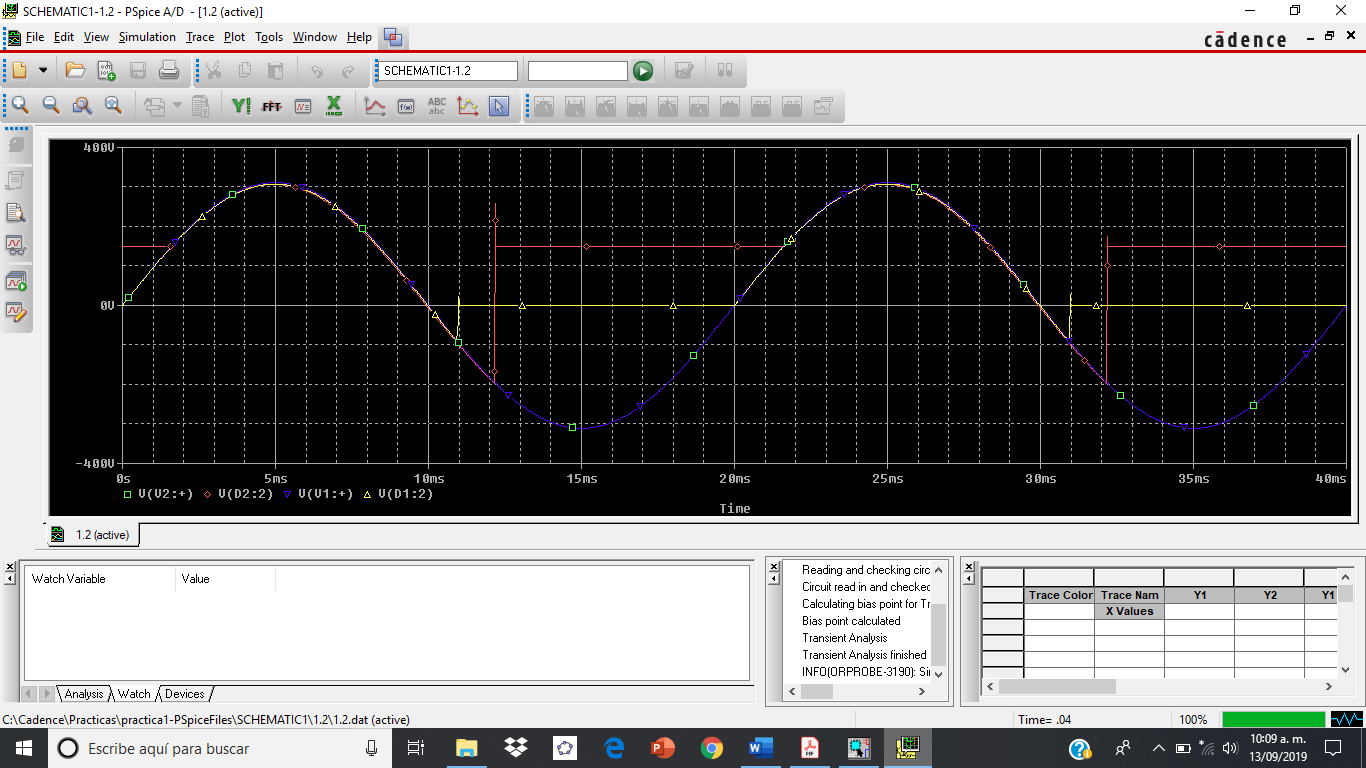
\includegraphics[scale=.25]{uno.png} $$

Se observa que la tension de salida no se anula hasta que no lo hace la corriente de carga, lo que significa que el diodo rectificador permanece polarizado en directo incluso durante una porcion del semiperiodo negativo de la tension de entrada.\\
Este hecho es debido a que la inductancia de salida se opone a variaciones bruscas de corriente, creando la sobre tension necesaria para mantener al diodo en conduccion hasta que la corriente sea nula.
\section{Rectificador monofasico en puente}
\subsection{Circuito}
$$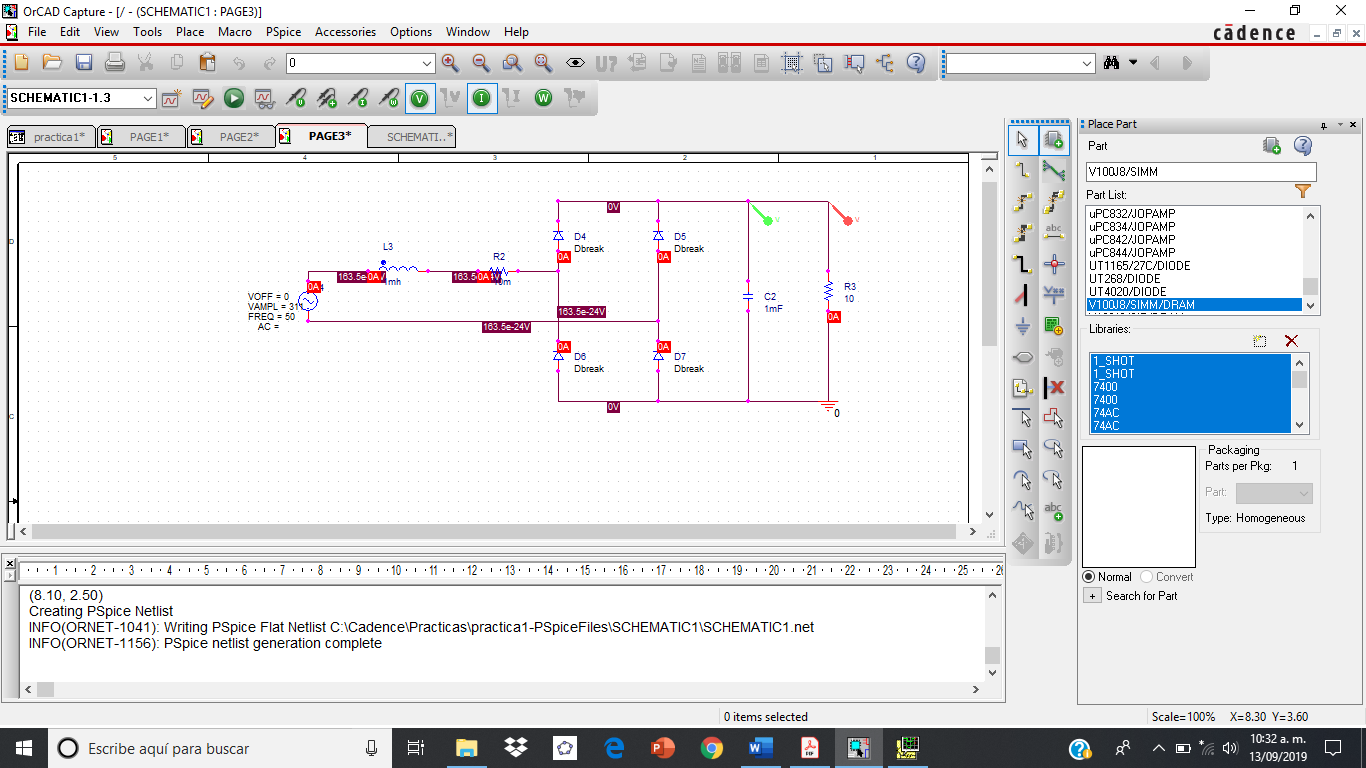
\includegraphics[scale=.25]{3.png} $$
\subsection{Onda}
$$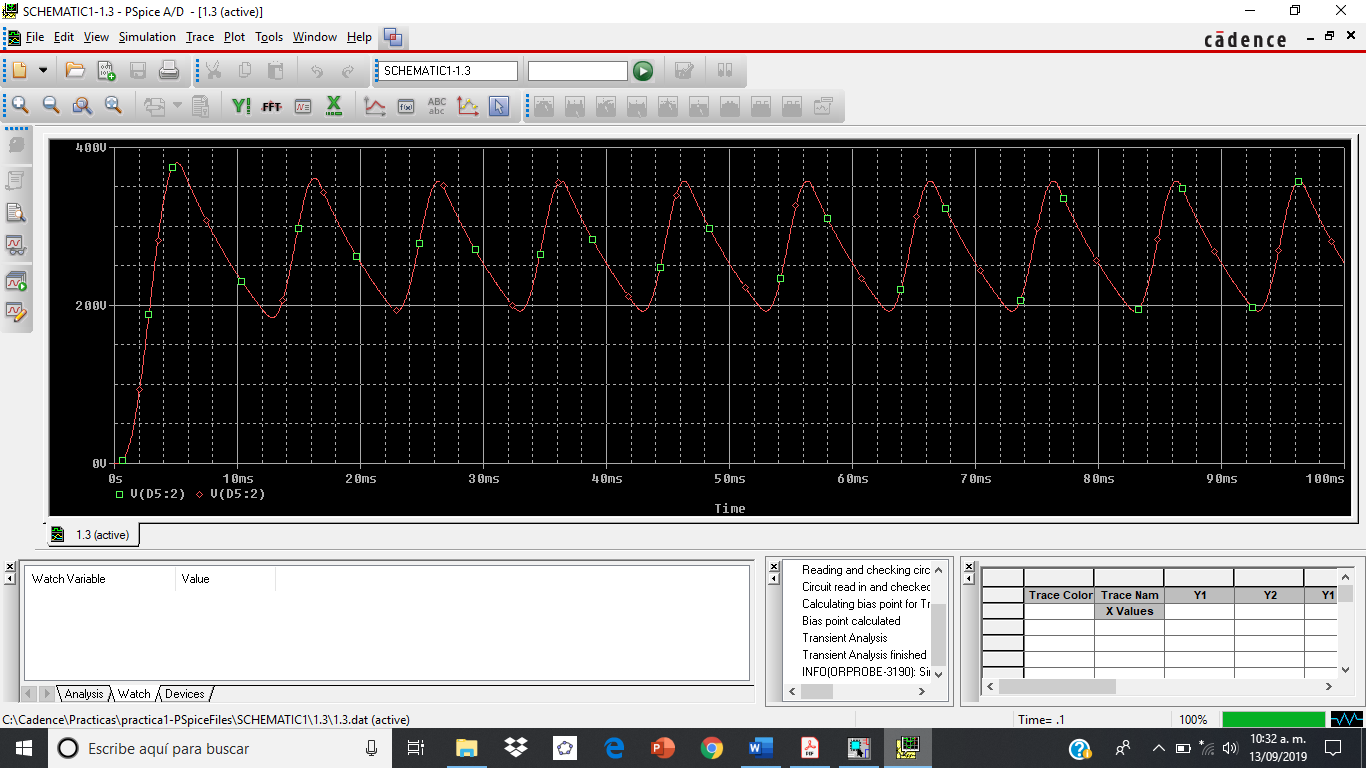
\includegraphics[scale=.25]{tres.png} $$

El circuito rectificador monofasico permite variar la componente de la tension de salida en funsion del troceado producido por una pareja de tiristores de acuerdo con el angulo de fase de disparo de los mismos.\\
La onda formada efectuara un analisis de fourier sobre la variable indicada, esto es, la corriente de entrada del rectificador.
\section{Circuito utilizado para el estudio de la tension PCC}
\subsection{Circuito }
$$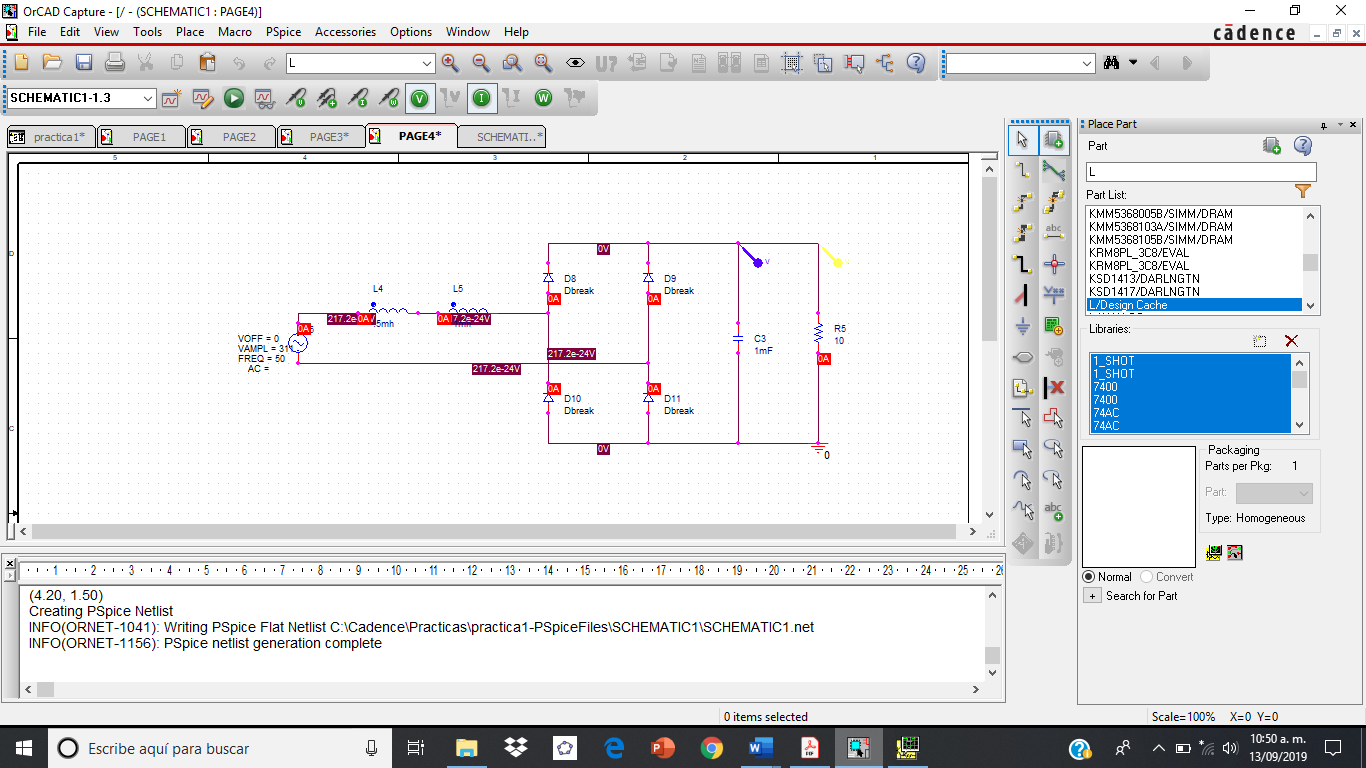
\includegraphics[scale=.25]{4.png} $$
\subsection{Onda}
$$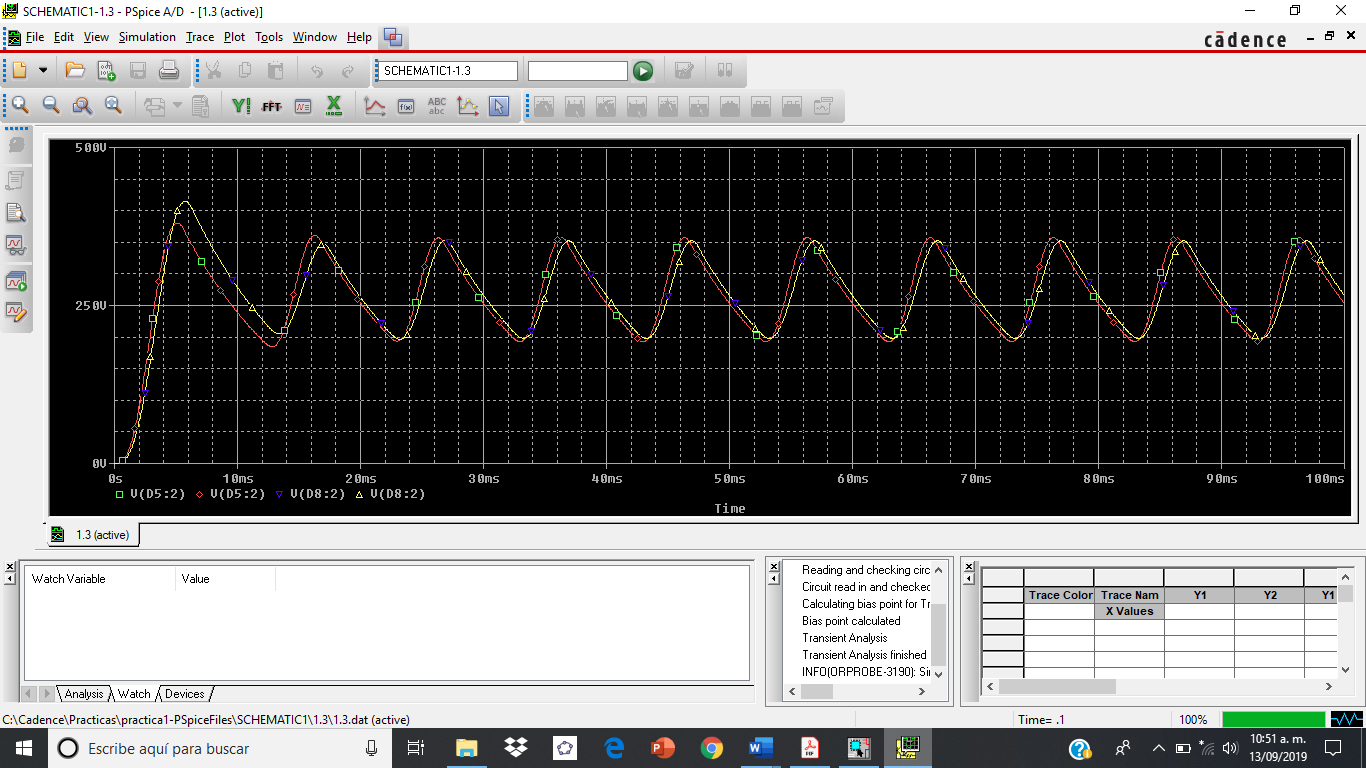
\includegraphics[scale=.25]{cuatro.png} $$

La primer bobina del circuito ,modeliza la inductancia de la linea de distribucion, tanto que la segunda bobina equivale a la inductancia que existe entre el PCC y el rectificador.\\
 
\section{Rectificador monofasico duplicador de tension}
\subsection{Circuito }
$$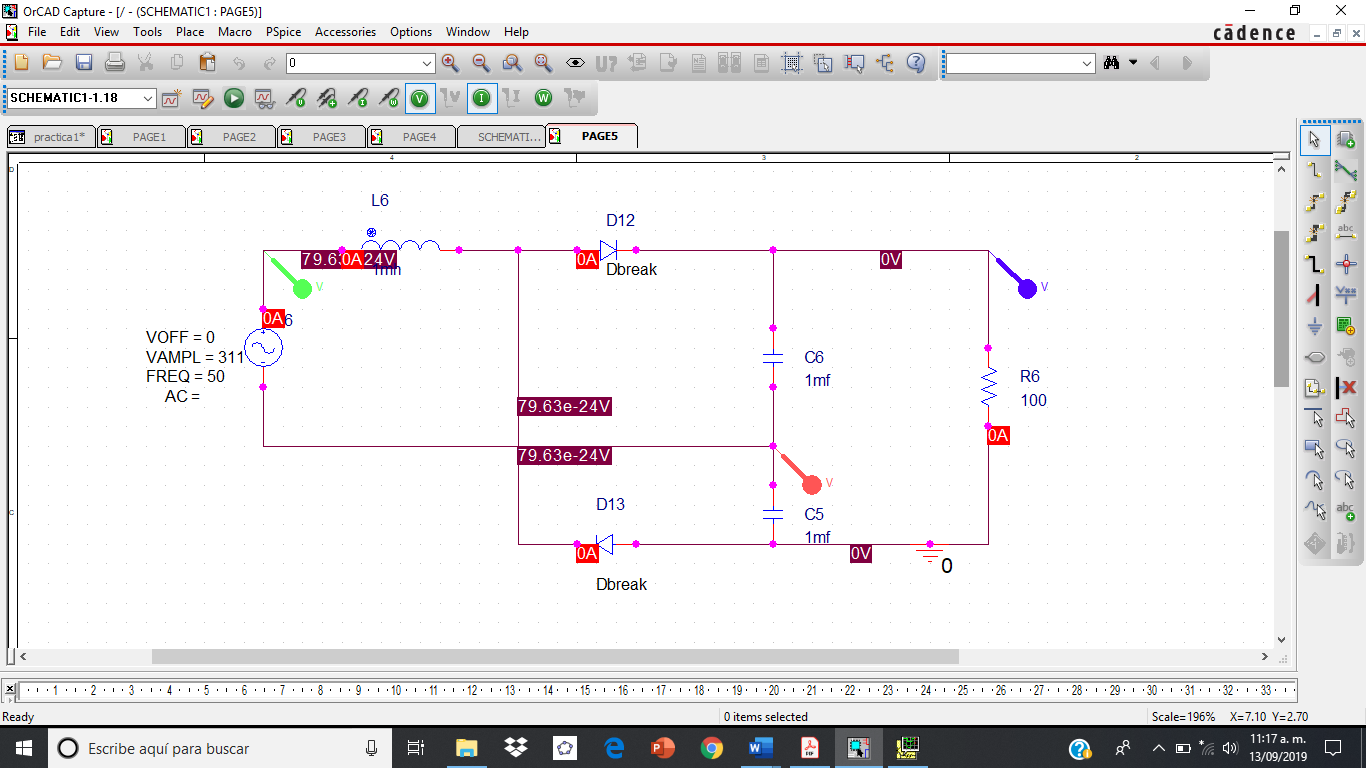
\includegraphics[scale=.25]{5.png} $$
\subsection{Onda}
$$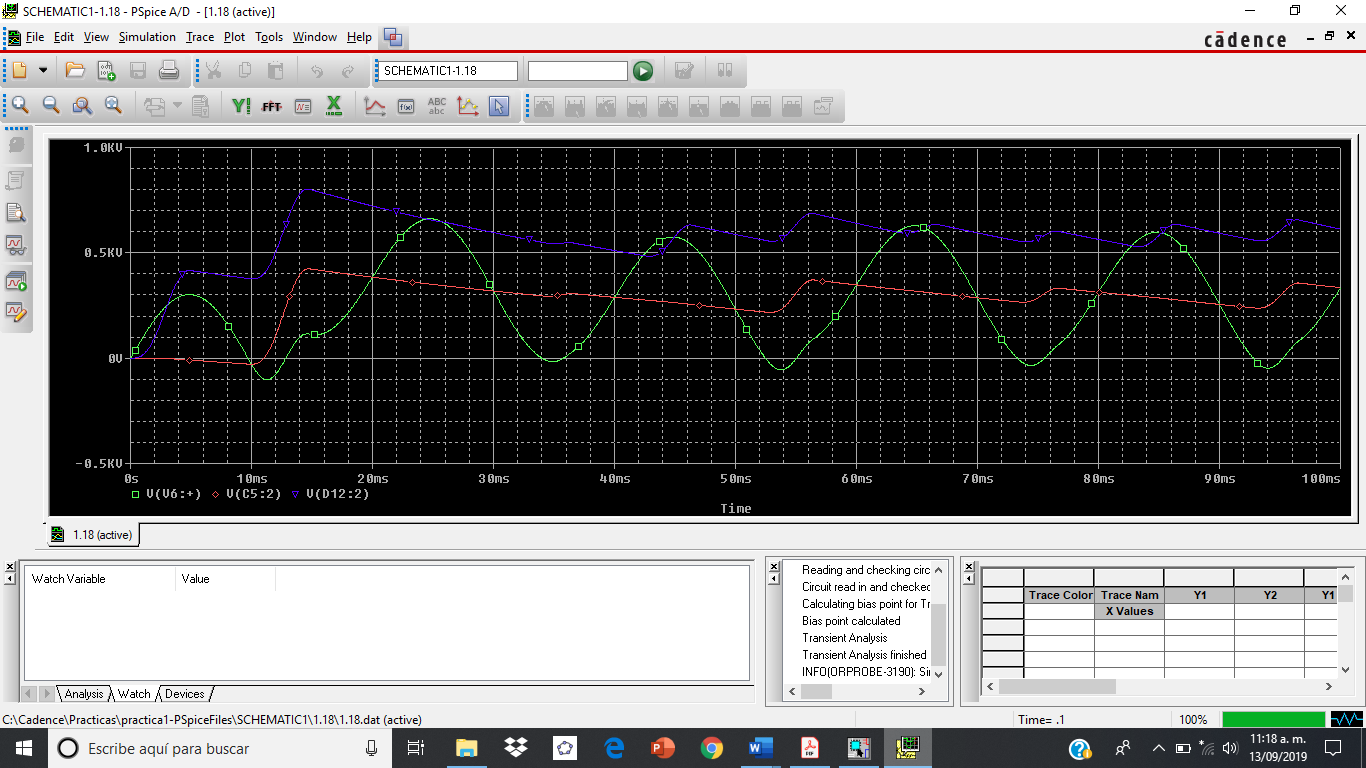
\includegraphics[scale=.25]{cinco.png} $$

Este circuito como su nombre lo menciona, su trabajo es obtener una tension de salida duplicada del que se obtiene al circuito anterior.\\ 
De esta manera es posible obtener tensiones en la etapa de continua sin la necesidad de utilizar un transformador que eleve la tension de entrada del rectificador.

\section{Rectificador Esquema de conexion de tres rectificadores monofasicos a una linea a 4 hilos}
\subsection{Circuito }
$$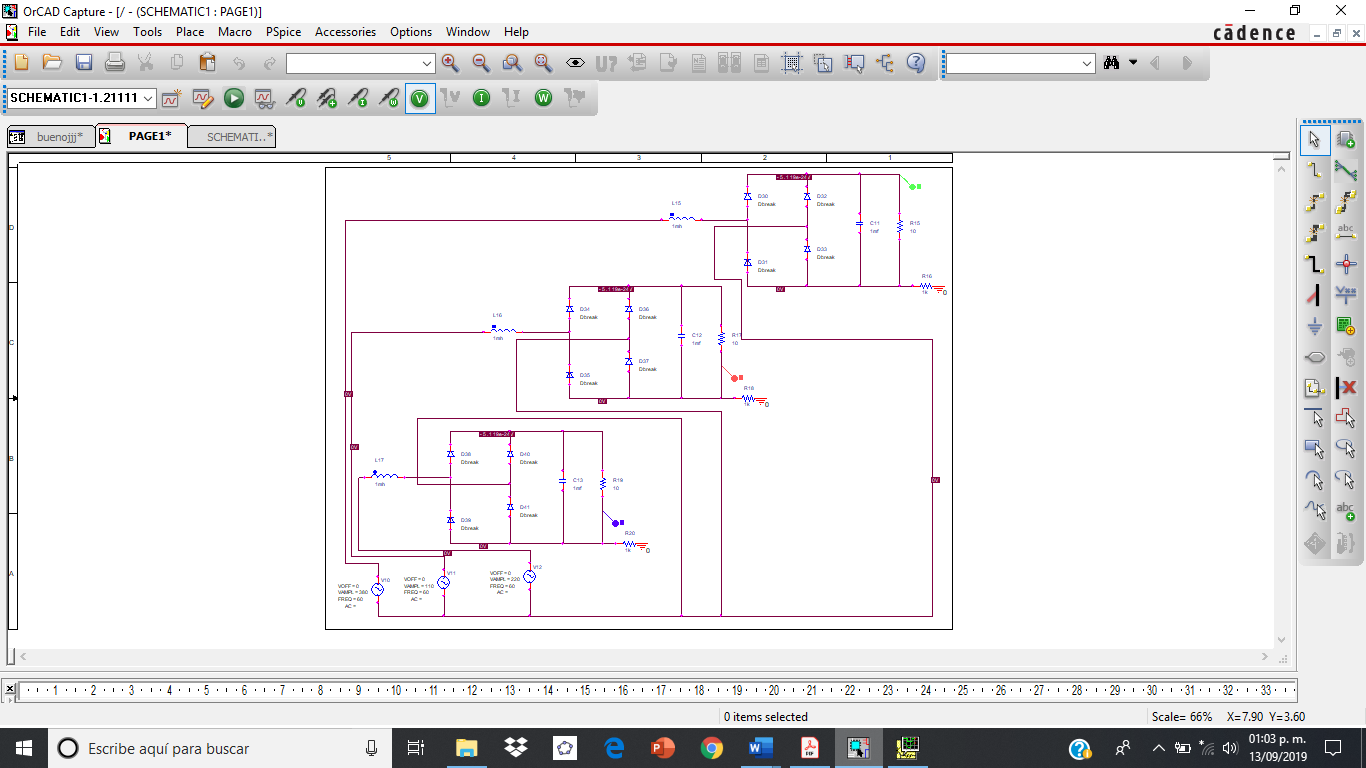
\includegraphics[scale=.25]{6.png} $$
\subsection{Onda}
$$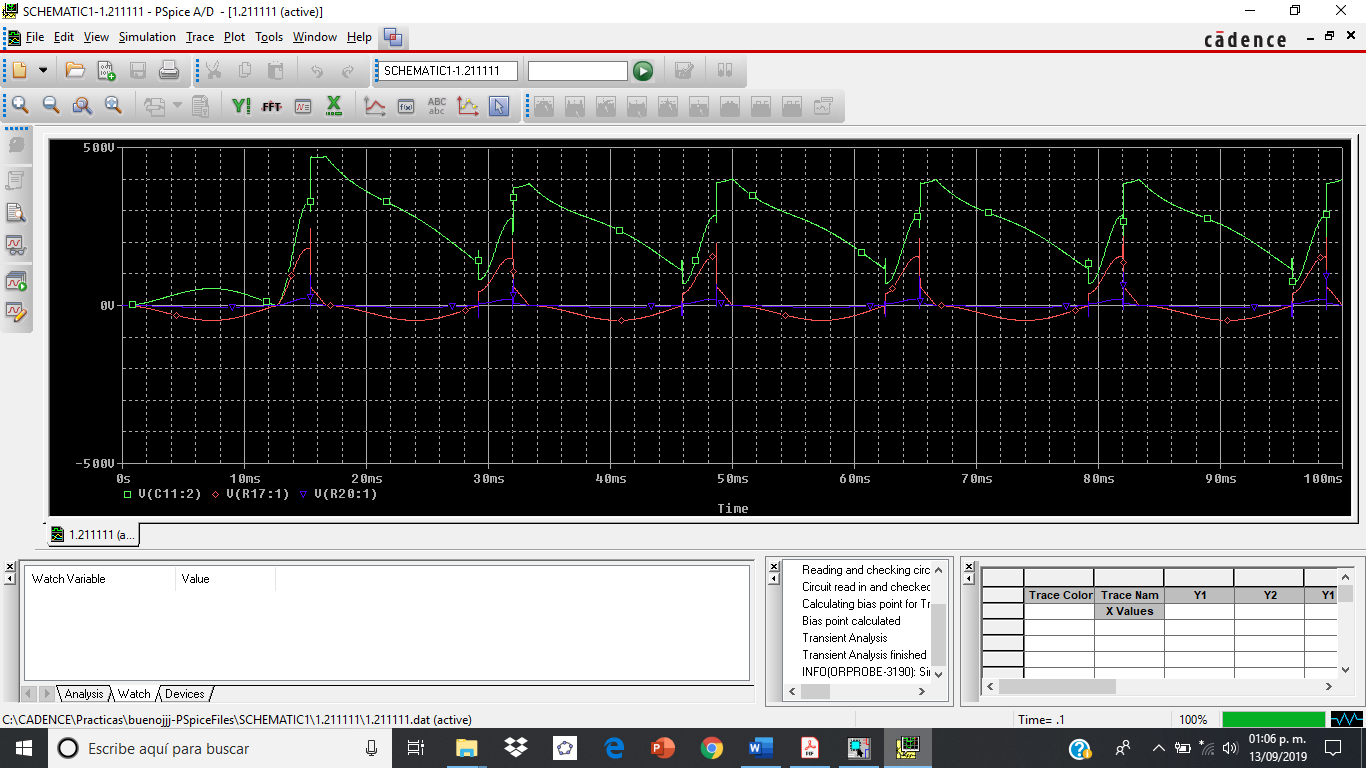
\includegraphics[scale=.25]{seis.png} $$

El rectificador trifasico cumple con la misma funcion que un rectificador monofasico, con la diferencia que con estos rectificadores son alimentados por fuentes trifasicas, por lo que son mas eficientes y pueden manejar grandes potencias, ya que su salida manejan menor rizado de la senal.
\section{Rectificador trifasico con filtro LC de salida}
\subsection{Circuito }
$$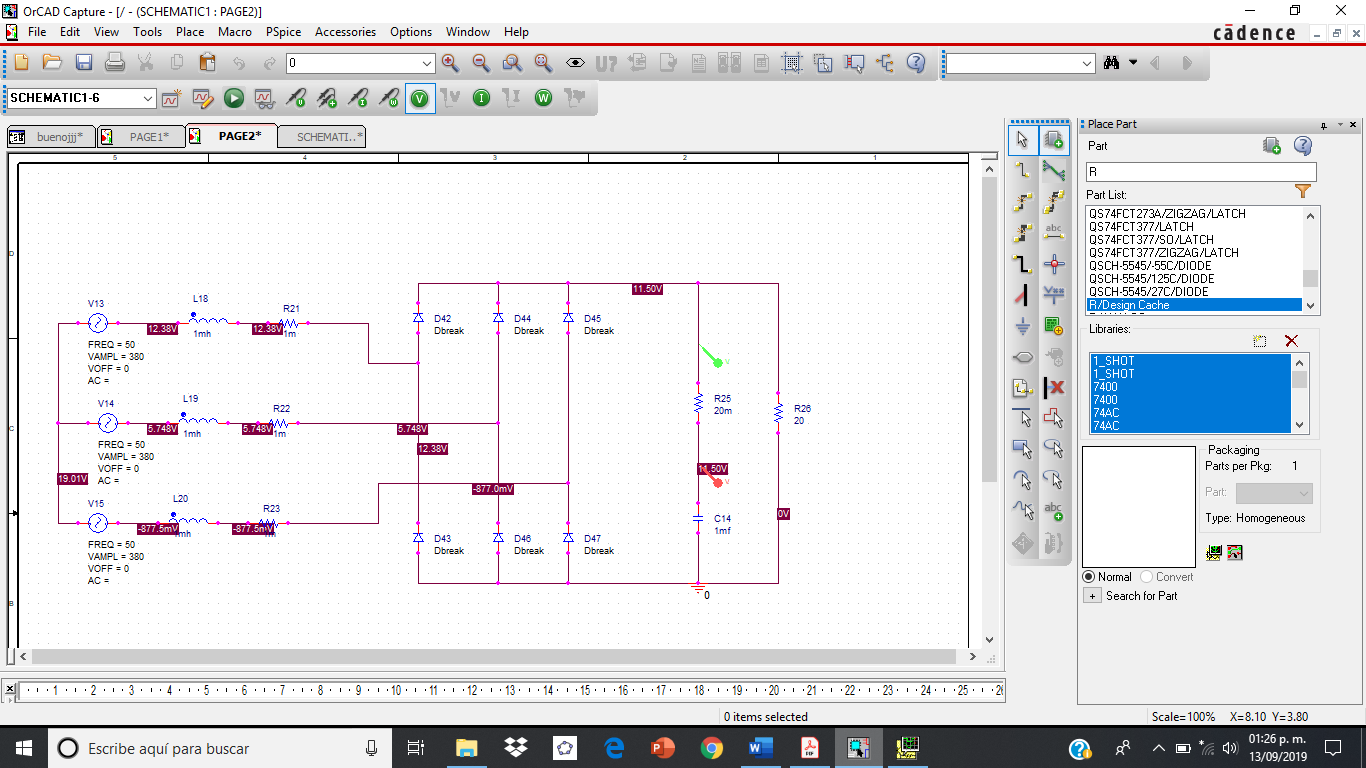
\includegraphics[scale=.25]{7.png} $$
\subsection{Onda}
$$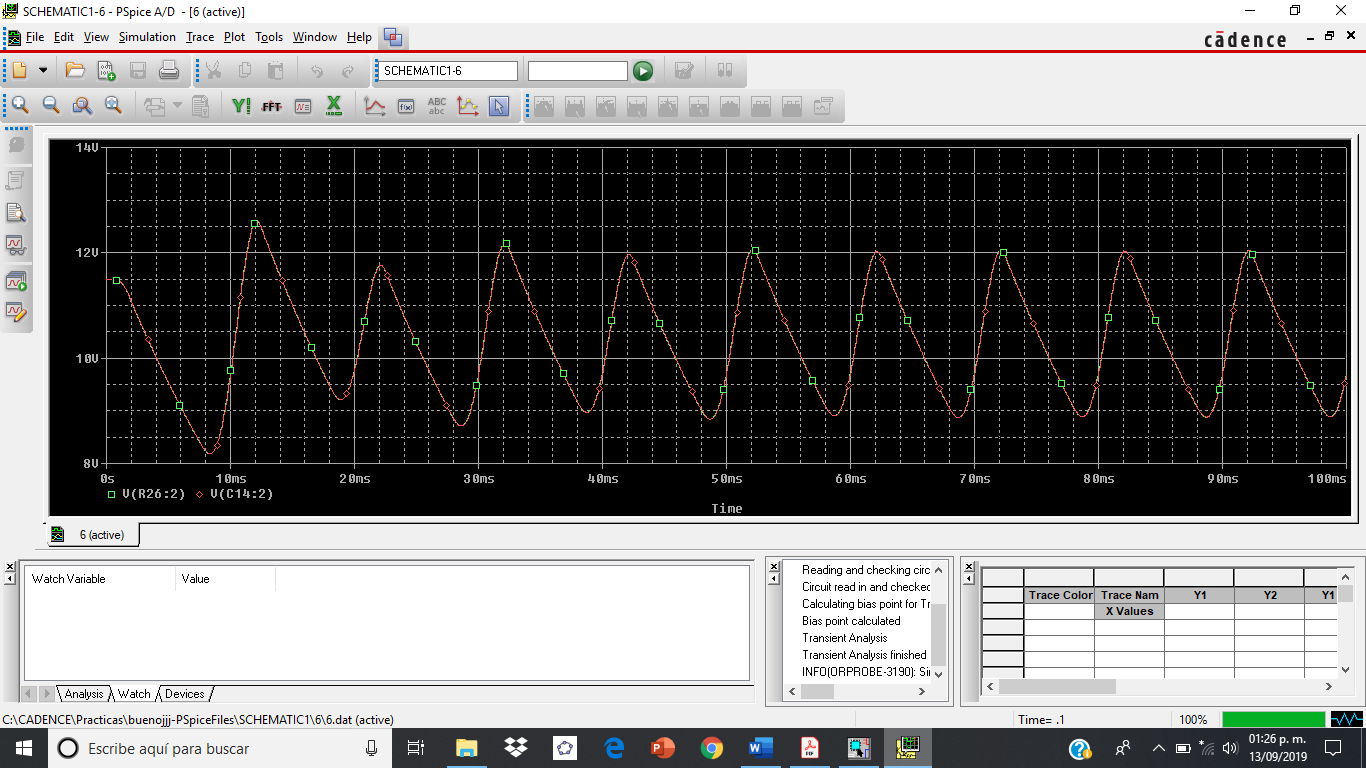
\includegraphics[scale=.25]{siete.png} $$

En este circuito vimos que cuando se utiliza una inductancia en la etapa de continua, se analiza como se evoluciona el factor de potencia cuando se modifica el valor de LF.
\section{Rectificador de conmutacion entre diodos}
\subsection{Circuito }
$$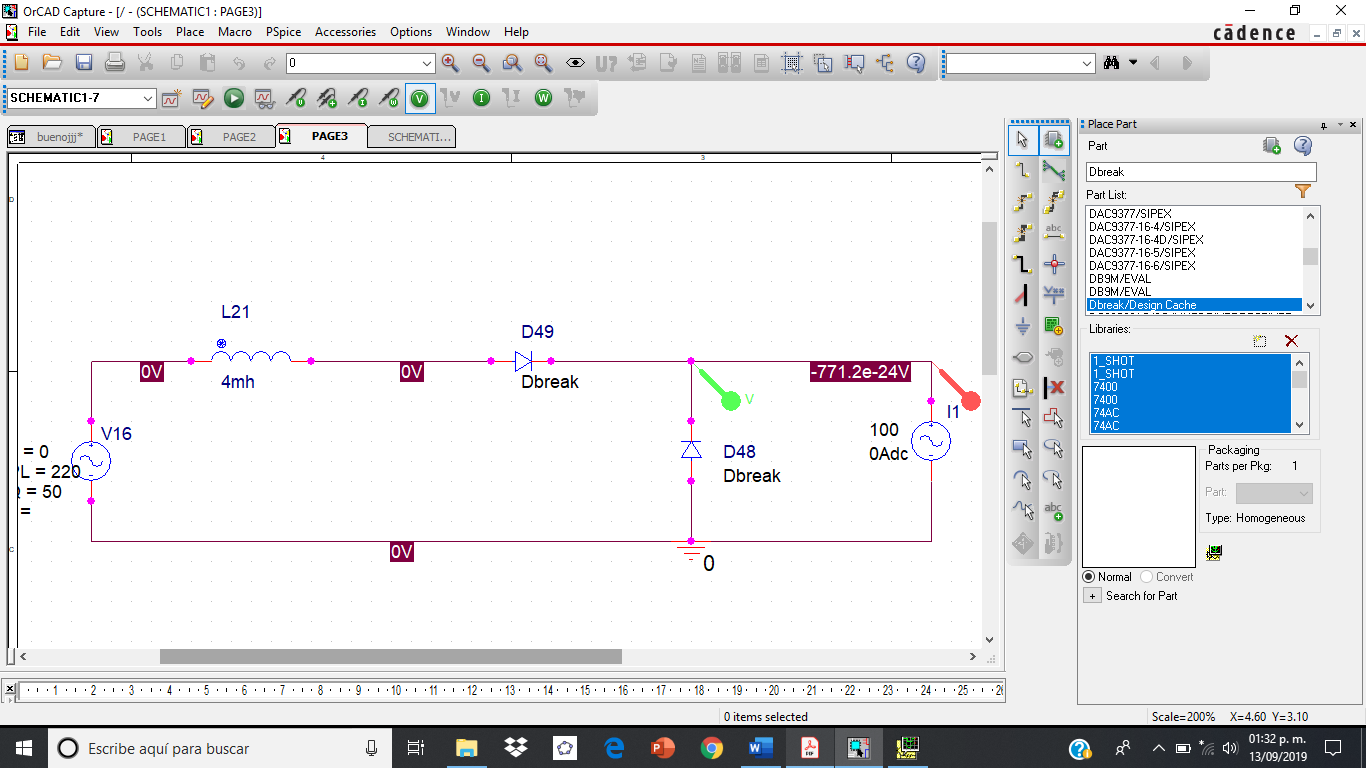
\includegraphics[scale=.25]{8.png} $$
\subsection{Onda}
$$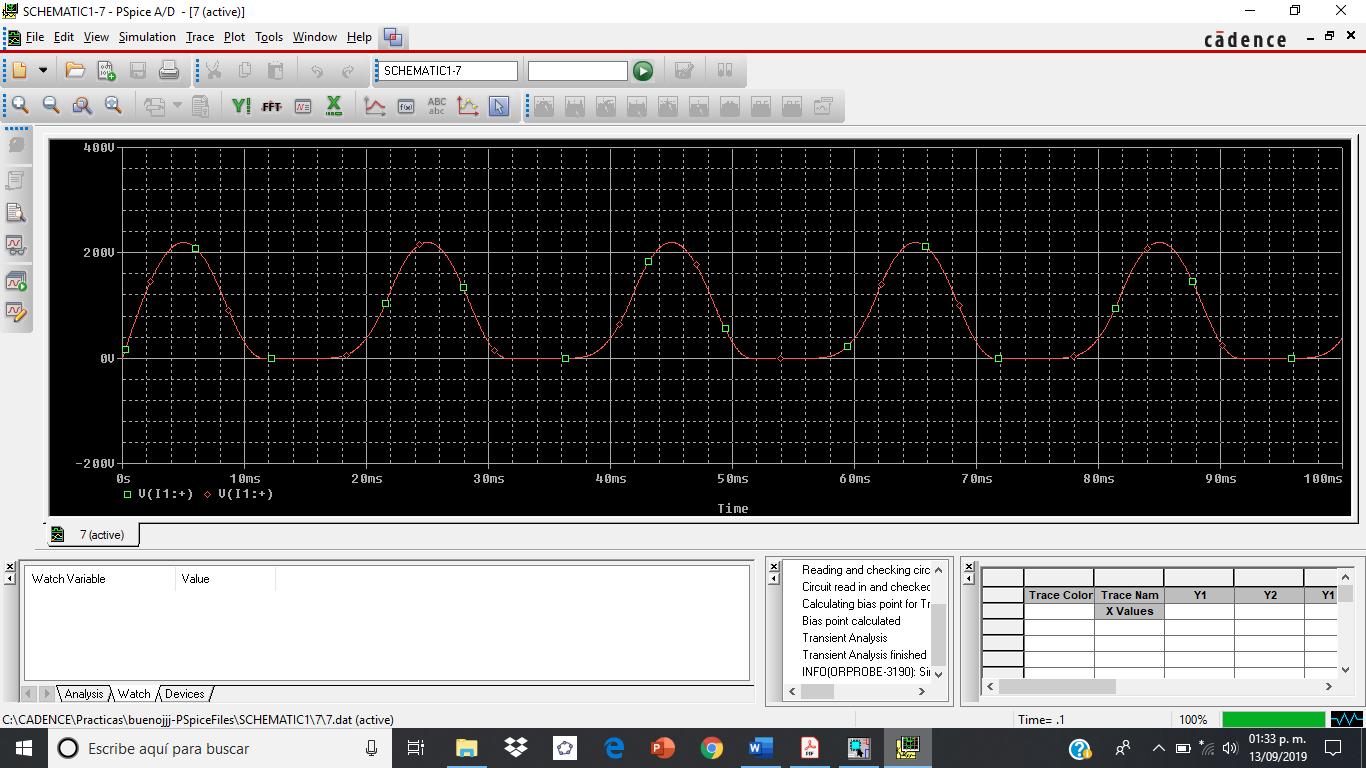
\includegraphics[scale=.25]{ocho.png} $$

En este circuito y en ausencia de inductancia de red, cuando la tension de entrada fuese positiva del primer diodo se pilarizaria en directo y conduciria en directo y conduciria.\\Esquema r
Por su parte el segundo diodoestaria polarizado en inversa y permaneceria en estado de bloqueo. 

\section{Conclusion}
En esta practica aprendimo a identficar los diferentes tipos de corrinte, ya se CC, CA, CD y tambien identificamos los diferentes tipos de fases, ya sea, monofasica, bifasica y/o trifasica, de igual forma los circuitos estrella y delta; todos con sus respectivos circuitos con sus ondas correspondientes
\end{document}